\section{Figures}
Figures are often the best way to convey dense blocks of information clearly and quickly. Always consider whether it is best to use a figure or a table. Consider \Cref{fig:Subfigs} and note some key aspects for a good figure:
\begin{itemize}
    \item Figure captions are always numbered and go \textbf{below} the figure. Furthermore, figures should not include a title as a caption alone is sufficient to describe the image.
    \item The font and marker sizes are appropriate and consistent with the rest of the report.
    \item The figure is saved in a vector format (.svg .pdf .eps) or in a high enough resolution such that it isn't pixelated.
    \item All axes are labelled and include units.
    \item The axes are scaled such that the data-points fit the space well and there isn't wasted white-space.
    \item Point markers, rather than lines are used to display measured data. Only \textit{continuous} data should be represented as a line.
    \item The figure is referred to in the main body of the text. No figure should be included unless it is directly referred to in your writing.
\end{itemize}

\begin{figure}
    \centering
    \begin{subfigure}[t]{0.49\columnwidth}
    \centering
        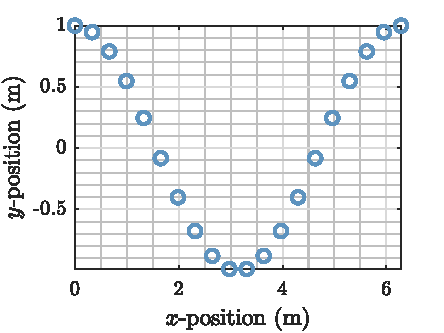
\includegraphics[width=\linewidth]{Images/Cos.pdf}
        \caption{Projectile 1}
        \label{fig:Projectile1}
    \end{subfigure}\hfill
    \begin{subfigure}[t]{0.49\columnwidth}
    \centering
        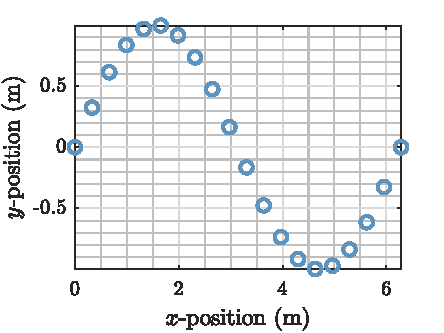
\includegraphics[width=\linewidth]{Images/Sin.pdf}
        \caption{Projectile 2}
        \label{fig:Projectile2}
    \end{subfigure}
    \caption{Trajectories of two projectiles as sub-figures.}
    \label{fig:ProjectilesSubFig}
\end{figure}

Note that sometimes it is better to combine figures where datasets are being compared. In the case of the two projectiles shown in \Cref{fig:Projectile1} and \Cref{fig:Projectile2}, the data is easier to compare when shown as in \Cref{fig:OneFig}. When multiple datasets are shown on a single figure, remember:
\begin{itemize}
    \item Use different markers and colours to differentiate between the datasets. It is best practice to always use different markers. Reports may be shown in black and white and differentiating only by colour is not enough.
    \item Include a legend that does not obscure the data-points and has sufficiently descriptive names.
\end{itemize}
By combining the the datasets we can enlarge the figure width to enhance clarity while taking up the same amount of page space.

\begin{figure}
    \centering
    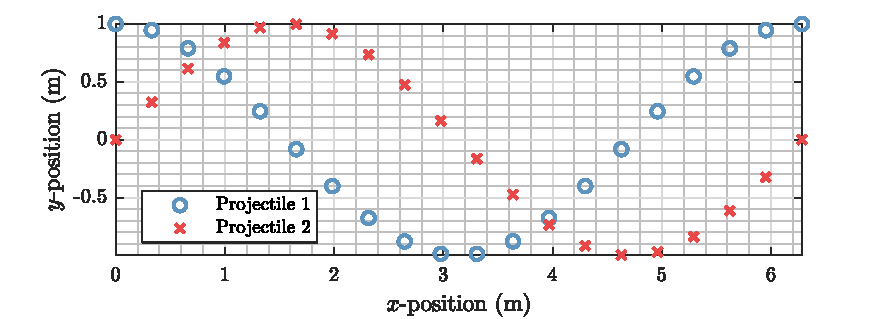
\includegraphics{Images/Both.pdf}
    \caption{Trajectories of two projectiles as a single figure.}
    \label{fig:OneFig}
\end{figure}